% !TEX encoding = UTF-8 Unicode
% !TEX program = xelatex

\documentclass{article}
	\usepackage[margin = 1in]{geometry}
	\usepackage{fontspec}
	\usepackage{tikz}
	\usepackage{listings}
\begin{document}



	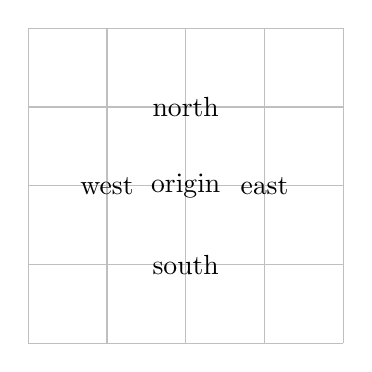
\begin{tikzpicture}
		\draw [lightgray] (-2, -2) grid (2, 2);
		                         \node at (0, 1) {north};
		\node at (-1, 0) {west}; \node at (0, 0) {origin}; \node at (1, 0) {east};
		                         \node at (0, -1) {south};
	\end{tikzpicture}



\fontspec{SourceCodePro-Regular}
\lstset{
	language=[latex]tex, tabsize=4,
	moredelim=*[s][\itshape]{$}{$},
	moredelim=*[s][\color{red!40!.}]{(}{)},
	moredelim=*[s][\color{green!30!.}]{[}{]},
	backgroundcolor=\color{blue!5},
	commentstyle=\color{.!80}\itshape,
	texcsstyle=*\color{blue!40!.},
	moretexcs={
		draw,node
	},
	deletetexcs={},
}
\lstinputlisting{node.tex}

\end{document}